% Options for packages loaded elsewhere
\PassOptionsToPackage{unicode}{hyperref}
\PassOptionsToPackage{hyphens}{url}
\documentclass[
  10pt,
]{article}
\usepackage{xcolor}
\usepackage[margin=0.6in]{geometry}
\usepackage{amsmath,amssymb}
\setcounter{secnumdepth}{-\maxdimen} % remove section numbering
\usepackage{iftex}
\ifPDFTeX
  \usepackage[T1]{fontenc}
  \usepackage[utf8]{inputenc}
  \usepackage{textcomp} % provide euro and other symbols
\else % if luatex or xetex
  \usepackage{unicode-math} % this also loads fontspec
  \defaultfontfeatures{Scale=MatchLowercase}
  \defaultfontfeatures[\rmfamily]{Ligatures=TeX,Scale=1}
\fi
\usepackage{lmodern}
\ifPDFTeX\else
  % xetex/luatex font selection
\fi
% Use upquote if available, for straight quotes in verbatim environments
\IfFileExists{upquote.sty}{\usepackage{upquote}}{}
\IfFileExists{microtype.sty}{% use microtype if available
  \usepackage[]{microtype}
  \UseMicrotypeSet[protrusion]{basicmath} % disable protrusion for tt fonts
}{}
\makeatletter
\@ifundefined{KOMAClassName}{% if non-KOMA class
  \IfFileExists{parskip.sty}{%
    \usepackage{parskip}
  }{% else
    \setlength{\parindent}{0pt}
    \setlength{\parskip}{6pt plus 2pt minus 1pt}}
}{% if KOMA class
  \KOMAoptions{parskip=half}}
\makeatother
\usepackage{color}
\usepackage{fancyvrb}
\newcommand{\VerbBar}{|}
\newcommand{\VERB}{\Verb[commandchars=\\\{\}]}
\DefineVerbatimEnvironment{Highlighting}{Verbatim}{commandchars=\\\{\}}
% Add ',fontsize=\small' for more characters per line
\usepackage{framed}
\definecolor{shadecolor}{RGB}{248,248,248}
\newenvironment{Shaded}{\begin{snugshade}}{\end{snugshade}}
\newcommand{\AlertTok}[1]{\textcolor[rgb]{0.94,0.16,0.16}{#1}}
\newcommand{\AnnotationTok}[1]{\textcolor[rgb]{0.56,0.35,0.01}{\textbf{\textit{#1}}}}
\newcommand{\AttributeTok}[1]{\textcolor[rgb]{0.13,0.29,0.53}{#1}}
\newcommand{\BaseNTok}[1]{\textcolor[rgb]{0.00,0.00,0.81}{#1}}
\newcommand{\BuiltInTok}[1]{#1}
\newcommand{\CharTok}[1]{\textcolor[rgb]{0.31,0.60,0.02}{#1}}
\newcommand{\CommentTok}[1]{\textcolor[rgb]{0.56,0.35,0.01}{\textit{#1}}}
\newcommand{\CommentVarTok}[1]{\textcolor[rgb]{0.56,0.35,0.01}{\textbf{\textit{#1}}}}
\newcommand{\ConstantTok}[1]{\textcolor[rgb]{0.56,0.35,0.01}{#1}}
\newcommand{\ControlFlowTok}[1]{\textcolor[rgb]{0.13,0.29,0.53}{\textbf{#1}}}
\newcommand{\DataTypeTok}[1]{\textcolor[rgb]{0.13,0.29,0.53}{#1}}
\newcommand{\DecValTok}[1]{\textcolor[rgb]{0.00,0.00,0.81}{#1}}
\newcommand{\DocumentationTok}[1]{\textcolor[rgb]{0.56,0.35,0.01}{\textbf{\textit{#1}}}}
\newcommand{\ErrorTok}[1]{\textcolor[rgb]{0.64,0.00,0.00}{\textbf{#1}}}
\newcommand{\ExtensionTok}[1]{#1}
\newcommand{\FloatTok}[1]{\textcolor[rgb]{0.00,0.00,0.81}{#1}}
\newcommand{\FunctionTok}[1]{\textcolor[rgb]{0.13,0.29,0.53}{\textbf{#1}}}
\newcommand{\ImportTok}[1]{#1}
\newcommand{\InformationTok}[1]{\textcolor[rgb]{0.56,0.35,0.01}{\textbf{\textit{#1}}}}
\newcommand{\KeywordTok}[1]{\textcolor[rgb]{0.13,0.29,0.53}{\textbf{#1}}}
\newcommand{\NormalTok}[1]{#1}
\newcommand{\OperatorTok}[1]{\textcolor[rgb]{0.81,0.36,0.00}{\textbf{#1}}}
\newcommand{\OtherTok}[1]{\textcolor[rgb]{0.56,0.35,0.01}{#1}}
\newcommand{\PreprocessorTok}[1]{\textcolor[rgb]{0.56,0.35,0.01}{\textit{#1}}}
\newcommand{\RegionMarkerTok}[1]{#1}
\newcommand{\SpecialCharTok}[1]{\textcolor[rgb]{0.81,0.36,0.00}{\textbf{#1}}}
\newcommand{\SpecialStringTok}[1]{\textcolor[rgb]{0.31,0.60,0.02}{#1}}
\newcommand{\StringTok}[1]{\textcolor[rgb]{0.31,0.60,0.02}{#1}}
\newcommand{\VariableTok}[1]{\textcolor[rgb]{0.00,0.00,0.00}{#1}}
\newcommand{\VerbatimStringTok}[1]{\textcolor[rgb]{0.31,0.60,0.02}{#1}}
\newcommand{\WarningTok}[1]{\textcolor[rgb]{0.56,0.35,0.01}{\textbf{\textit{#1}}}}
\usepackage{graphicx}
\makeatletter
\newsavebox\pandoc@box
\newcommand*\pandocbounded[1]{% scales image to fit in text height/width
  \sbox\pandoc@box{#1}%
  \Gscale@div\@tempa{\textheight}{\dimexpr\ht\pandoc@box+\dp\pandoc@box\relax}%
  \Gscale@div\@tempb{\linewidth}{\wd\pandoc@box}%
  \ifdim\@tempb\p@<\@tempa\p@\let\@tempa\@tempb\fi% select the smaller of both
  \ifdim\@tempa\p@<\p@\scalebox{\@tempa}{\usebox\pandoc@box}%
  \else\usebox{\pandoc@box}%
  \fi%
}
% Set default figure placement to htbp
\def\fps@figure{htbp}
\makeatother
\setlength{\emergencystretch}{3em} % prevent overfull lines
\providecommand{\tightlist}{%
  \setlength{\itemsep}{0pt}\setlength{\parskip}{0pt}}
\usepackage{bookmark}
\IfFileExists{xurl.sty}{\usepackage{xurl}}{} % add URL line breaks if available
\urlstyle{same}
\hypersetup{
  pdftitle={FormIOr Cheat Sheet},
  hidelinks,
  pdfcreator={LaTeX via pandoc}}

\title{FormIOr Cheat Sheet}
\author{}
\date{\vspace{-2.5em}}

\begin{document}
\maketitle

\section{Core Workflow (Most Common
Path)}\label{core-workflow-most-common-path}

\textbf{Goal:} Download -\textgreater{} Flatten -\textgreater{} Clean
-\textgreater{} Diagnose -\textgreater{} Export

\includegraphics[width=1\linewidth]{assets/core-workflow}

\textbf{CHEF credentials (quick visual):} API key and Form ID are in the
form's \textbf{Manage} page.\\
Form ID is the alphanumeric code after \texttt{=} in the Manage page
URL.

\includegraphics[width=1\linewidth]{assets/API}
\includegraphics[width=1\linewidth]{assets/FormID}

Default CHEF base URL used by FormIOr:

\begin{verbatim}
https://submit.digital.gov.bc.ca/app/api/v1
\end{verbatim}

Note (CHEF): Metadata/schema endpoints may live at \texttt{/api/v1}.
FormIOr will automatically retry the alternate base for metadata/schema
requests when needed.

\begin{enumerate}
\def\labelenumi{\arabic{enumi}.}
\tightlist
\item
  \textbf{Download responses}
\end{enumerate}

\begin{Shaded}
\begin{Highlighting}[]
\NormalTok{raw }\OtherTok{\textless{}{-}} \FunctionTok{GetResponses}\NormalTok{(}\AttributeTok{form\_id =} \StringTok{"YOUR\_FORM\_ID"}\NormalTok{)}
\end{Highlighting}
\end{Shaded}

Tip: Many cleaning helpers return a list with \texttt{out\$data} (the
cleaned \texttt{data.frame}) and, when \texttt{return\_flat\ =\ TRUE},
\texttt{out\$flat} (an updated FlattenSubmissions-style list). In this
cheat sheet we keep both:

\begin{itemize}
\tightlist
\item
  \texttt{df} = the cleaned \texttt{data.frame} you typically
  analyze/export
\item
  \texttt{flat} = the updated FlattenSubmissions list (when you need
  \texttt{FlatResponses} + metadata)
\end{itemize}

\begin{enumerate}
\def\labelenumi{\arabic{enumi}.}
\setcounter{enumi}{1}
\tightlist
\item
  \textbf{Flatten nested responses}
\end{enumerate}

\begin{Shaded}
\begin{Highlighting}[]
\NormalTok{flat\_raw }\OtherTok{\textless{}{-}} \FunctionTok{FlattenSubmissions}\NormalTok{(raw)}
\NormalTok{df }\OtherTok{\textless{}{-}}\NormalTok{ flat\_raw}\SpecialCharTok{$}\NormalTok{FlatResponses}
\end{Highlighting}
\end{Shaded}

\begin{enumerate}
\def\labelenumi{\arabic{enumi}.}
\setcounter{enumi}{2}
\tightlist
\item
  \textbf{Normalize column names (recommended)}
\end{enumerate}

\begin{Shaded}
\begin{Highlighting}[]
\NormalTok{norm }\OtherTok{\textless{}{-}} \FunctionTok{NormalizeColumnNames}\NormalTok{(flat\_raw, }\AttributeTok{return\_flat =} \ConstantTok{TRUE}\NormalTok{)}
\NormalTok{flat }\OtherTok{\textless{}{-}}\NormalTok{ norm}\SpecialCharTok{$}\NormalTok{flat}
\NormalTok{df }\OtherTok{\textless{}{-}}\NormalTok{ norm}\SpecialCharTok{$}\NormalTok{data}
\end{Highlighting}
\end{Shaded}

\begin{enumerate}
\def\labelenumi{\arabic{enumi}.}
\setcounter{enumi}{3}
\tightlist
\item
  \textbf{Deduplicate (optional)}
\end{enumerate}

\begin{Shaded}
\begin{Highlighting}[]
\NormalTok{dedup }\OtherTok{\textless{}{-}} \FunctionTok{DeduplicateSubmissions}\NormalTok{(flat, }\AttributeTok{id\_col =} \StringTok{"form\_submissionid"}\NormalTok{, }\AttributeTok{return\_flat =} \ConstantTok{TRUE}\NormalTok{)}
\NormalTok{flat }\OtherTok{\textless{}{-}}\NormalTok{ dedup}\SpecialCharTok{$}\NormalTok{flat}
\NormalTok{df }\OtherTok{\textless{}{-}}\NormalTok{ dedup}\SpecialCharTok{$}\NormalTok{data}
\end{Highlighting}
\end{Shaded}

\begin{enumerate}
\def\labelenumi{\arabic{enumi}.}
\setcounter{enumi}{4}
\tightlist
\item
  \textbf{Resolve repeated answers (optional)}
\end{enumerate}

\begin{Shaded}
\begin{Highlighting}[]
\NormalTok{resolved }\OtherTok{\textless{}{-}} \FunctionTok{ResolveRepeats}\NormalTok{(flat, }\AttributeTok{id\_col =} \StringTok{"form\_submissionid"}\NormalTok{, }\AttributeTok{return\_flat =} \ConstantTok{TRUE}\NormalTok{)}
\NormalTok{flat }\OtherTok{\textless{}{-}}\NormalTok{ resolved}\SpecialCharTok{$}\NormalTok{flat}
\NormalTok{df }\OtherTok{\textless{}{-}}\NormalTok{ resolved}\SpecialCharTok{$}\NormalTok{data}
\end{Highlighting}
\end{Shaded}

\begin{enumerate}
\def\labelenumi{\arabic{enumi}.}
\setcounter{enumi}{5}
\tightlist
\item
  \textbf{Create a codebook}
\end{enumerate}

\begin{Shaded}
\begin{Highlighting}[]
\NormalTok{codebook }\OtherTok{\textless{}{-}} \FunctionTok{MakeCodebook}\NormalTok{(df)}
\CommentTok{\# Optional: include labels from the form schema}
\CommentTok{\# form\_meta \textless{}{-} GetFormMetadata(form\_id = "your{-}form{-}id", api\_key = "your{-}api{-}key")}
\CommentTok{\# codebook \textless{}{-} MakeCodebook(df, form = form\_meta, include = "all")}
\end{Highlighting}
\end{Shaded}

\begin{enumerate}
\def\labelenumi{\arabic{enumi}.}
\setcounter{enumi}{6}
\tightlist
\item
  \textbf{Run quick diagnostics}
\end{enumerate}

\begin{Shaded}
\begin{Highlighting}[]
\NormalTok{summary\_age }\OtherTok{\textless{}{-}} \FunctionTok{SummaryByField}\NormalTok{(df, }\AttributeTok{field =} \StringTok{"age"}\NormalTok{)}
\FunctionTok{PlotHistogram}\NormalTok{(df, }\StringTok{"age"}\NormalTok{)}
\FunctionTok{PlotBarSummary}\NormalTok{(df, }\StringTok{"program"}\NormalTok{)}
\end{Highlighting}
\end{Shaded}

\begin{enumerate}
\def\labelenumi{\arabic{enumi}.}
\setcounter{enumi}{7}
\tightlist
\item
  \textbf{Export to Excel}
\end{enumerate}

\begin{Shaded}
\begin{Highlighting}[]
\NormalTok{sheets }\OtherTok{\textless{}{-}} \FunctionTok{list}\NormalTok{(}
  \AttributeTok{Raw\_Flattened =}\NormalTok{ flat\_raw}\SpecialCharTok{$}\NormalTok{FlatResponses,}
  \AttributeTok{Cleaned\_Data =}\NormalTok{ df,}
  \AttributeTok{Codebook =}\NormalTok{ codebook,}
  \AttributeTok{Summary\_Age =}\NormalTok{ summary\_age}\SpecialCharTok{$}\NormalTok{summary}
\NormalTok{)}
\FunctionTok{ExportToExcel}\NormalTok{(sheets, }\AttributeTok{path =} \StringTok{"FormIOr\_output.xlsx"}\NormalTok{, }\AttributeTok{overwrite =} \ConstantTok{TRUE}\NormalTok{)}
\end{Highlighting}
\end{Shaded}

\section{Helpful Extras (Common
Add-Ons)}\label{helpful-extras-common-add-ons}

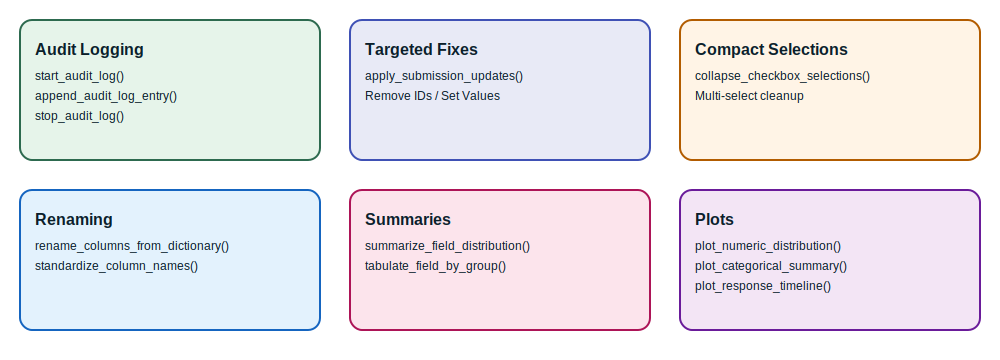
\includegraphics[width=1\linewidth]{assets/helpers-grid}

\textbf{Audit logging (highly recommended)}

\begin{Shaded}
\begin{Highlighting}[]
\FunctionTok{StartAuditLog}\NormalTok{(}\StringTok{"audit\_log.csv"}\NormalTok{)}
\FunctionTok{WriteAuditLog}\NormalTok{(}\StringTok{"flatten"}\NormalTok{, }\AttributeTok{details =} \StringTok{"Flattened submissions"}\NormalTok{)}
\FunctionTok{StopAuditLog}\NormalTok{()}
\end{Highlighting}
\end{Shaded}

\textbf{Targeted adjustments}

\begin{Shaded}
\begin{Highlighting}[]
\NormalTok{updates }\OtherTok{\textless{}{-}} \FunctionTok{data.frame}\NormalTok{(}
  \AttributeTok{id =} \StringTok{"sub\_020"}\NormalTok{,}
  \AttributeTok{column =} \StringTok{"region"}\NormalTok{,}
  \AttributeTok{value =} \StringTok{"North"}\NormalTok{,}
  \AttributeTok{stringsAsFactors =} \ConstantTok{FALSE}
\NormalTok{)}

\NormalTok{adj }\OtherTok{\textless{}{-}} \FunctionTok{AdjustSubmissions}\NormalTok{(}
\NormalTok{  flat,}
  \AttributeTok{id\_col =} \StringTok{"form\_submissionid"}\NormalTok{,}
  \AttributeTok{delete\_ids =} \FunctionTok{c}\NormalTok{(}\StringTok{"sub\_001"}\NormalTok{, }\StringTok{"sub\_017"}\NormalTok{),}
  \AttributeTok{updates =}\NormalTok{ updates,}
  \AttributeTok{return\_flat =} \ConstantTok{TRUE}
\NormalTok{)}
\NormalTok{flat }\OtherTok{\textless{}{-}}\NormalTok{ adj}\SpecialCharTok{$}\NormalTok{flat}
\NormalTok{df }\OtherTok{\textless{}{-}}\NormalTok{ adj}\SpecialCharTok{$}\NormalTok{data}
\end{Highlighting}
\end{Shaded}

\textbf{Compact multi-select columns}

\begin{Shaded}
\begin{Highlighting}[]
\NormalTok{comp }\OtherTok{\textless{}{-}} \FunctionTok{CompactSelections}\NormalTok{(flat, }\AttributeTok{return\_flat =} \ConstantTok{TRUE}\NormalTok{)}
\NormalTok{flat }\OtherTok{\textless{}{-}}\NormalTok{ comp}\SpecialCharTok{$}\NormalTok{flat}
\NormalTok{df }\OtherTok{\textless{}{-}}\NormalTok{ comp}\SpecialCharTok{$}\NormalTok{data}
\CommentTok{\# Optional: change the separator used to detect checkbox groups}
\CommentTok{\# flat \textless{}{-} CompactSelections(flat, sep = "{-}")}
\end{Highlighting}
\end{Shaded}

\textbf{Rename columns}

\begin{Shaded}
\begin{Highlighting}[]
\FunctionTok{RenameCols}\NormalTok{(flat)}
\end{Highlighting}
\end{Shaded}

\textbf{Cross-tab summaries}

\begin{Shaded}
\begin{Highlighting}[]
\FunctionTok{CrossTab}\NormalTok{(df, }\AttributeTok{row =} \StringTok{"region"}\NormalTok{, }\AttributeTok{col =} \StringTok{"program"}\NormalTok{)}
\end{Highlighting}
\end{Shaded}

\textbf{Response timelines}

\begin{Shaded}
\begin{Highlighting}[]
\FunctionTok{ResponseTimeline}\NormalTok{(df, }\AttributeTok{date\_col =} \StringTok{"created"}\NormalTok{)}
\FunctionTok{PlotResponseTimeline}\NormalTok{(df, }\AttributeTok{date\_col =} \StringTok{"created"}\NormalTok{)}
\end{Highlighting}
\end{Shaded}

\textbf{Pre/post comparability + suspicious responses}

\begin{Shaded}
\begin{Highlighting}[]
\FunctionTok{data}\NormalTok{(}\StringTok{"SuspiciousSurveyDemo"}\NormalTok{, }\AttributeTok{package =} \StringTok{"FormIOr"}\NormalTok{)}

\NormalTok{risk }\OtherTok{\textless{}{-}} \FunctionTok{FlagSuspiciousSubmissions}\NormalTok{(}
\NormalTok{  SuspiciousSurveyDemo,}
  \AttributeTok{id\_col =} \StringTok{"submissionId"}\NormalTok{,}
  \AttributeTok{time\_col =} \StringTok{"created"}\NormalTok{,}
  \AttributeTok{cutoff\_time =} \StringTok{"2026{-}01{-}06 00:00:00"}\NormalTok{,}
  \AttributeTok{group\_action =} \StringTok{"split\_only"}\NormalTok{,}
  \AttributeTok{action =} \StringTok{"flag\_only"}
\NormalTok{)}

\NormalTok{risk}\SpecialCharTok{$}\NormalTok{comparability}\SpecialCharTok{$}\NormalTok{non\_comparable}
\FunctionTok{head}\NormalTok{(risk}\SpecialCharTok{$}\NormalTok{flags)}
\end{Highlighting}
\end{Shaded}

\section{Wizard (Automated Workflow)}\label{wizard-automated-workflow}

\begin{Shaded}
\begin{Highlighting}[]
\NormalTok{out }\OtherTok{\textless{}{-}} \FunctionTok{FormIOrWorkflow}\NormalTok{()}
\end{Highlighting}
\end{Shaded}

This will: - create an output folder - start or reuse an audit log -
download, flatten, clean, diagnose, and export - save a plan so you can
replay the workflow later

\section{Quick Reference: Key
Functions}\label{quick-reference-key-functions}

\textbf{Download} - \texttt{GetResponses()} - \texttt{GetSubmissions()}
- \texttt{GetFormMetadata()}

\textbf{Flatten \& Clean} - \texttt{FlattenSubmissions()} -
\texttt{NormalizeColumnNames()} - \texttt{DeduplicateSubmissions()} -
\texttt{ResolveRepeats()} - \texttt{CompactSelections()} -
\texttt{AdjustSubmissions()}

\textbf{Diagnostics} - \texttt{MakeCodebook()} -
\texttt{SummaryByField()} - \texttt{CrossTab()} -
\texttt{PlotHistogram()} - \texttt{PlotBarSummary()} -
\texttt{PlotWordcloud()} - \texttt{PlotResponseTimeline()} -
\texttt{FlagSuspiciousSubmissions()}

\textbf{Bundled Demo Data} - \texttt{SuspiciousSurveyDemo}

\textbf{Export \& Logging} - \texttt{ExportToExcel()} -
\texttt{StartAuditLog()} - \texttt{WriteAuditLog()} -
\texttt{StopAuditLog()}

\end{document}
